\documentclass{article}
\usepackage[UTF8]{ctex}
\usepackage{amsmath,mathtools,geometry,pgfplots,float,mathrsfs,caption,enumerate}
\pgfplotsset{compat=1.15}
\usetikzlibrary{arrows}
\geometry{scale=0.7}

\title{每日一题(19.1)}
\author{\kaishu 程昊一}
\date{2022年5月31日}

\begin{document}
\maketitle
\begin{enumerate}
	\renewcommand{\labelenumi}{\textbf{\theenumi. }}
	\item 如图, 平面内有正$\triangle ABC$, 正$\triangle CDE$, 正$\triangle EHK$, 且$D$为$AK$中点. 求证: $\triangle BHD$为正三角形.(\kaishu 第15届全俄奥林匹克题)
	\begin{figure}[H]
		\flushright
		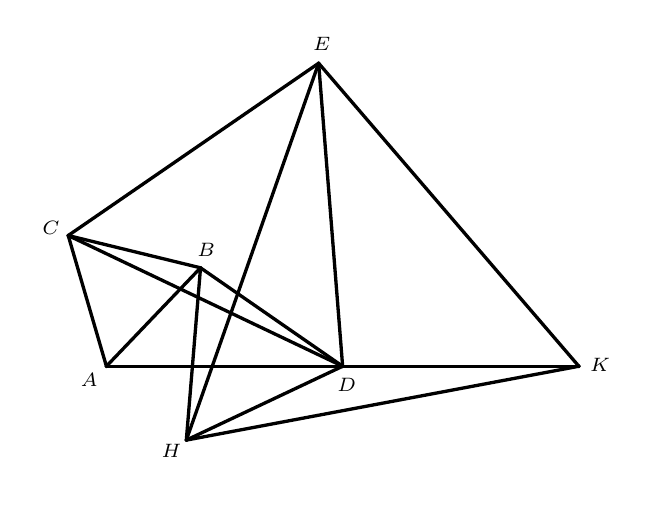
\begin{tikzpicture}[line cap=round,line join=round,>=triangle 45,x=1.0cm,y=1.0cm]
			\clip(-1.,-1.4) rectangle (6.5,4.3);
			\draw [line width=1.2pt] (0.,0.)-- (1.195216331374773,1.250170518894102);
			\draw [line width=1.2pt] (-0.48507126273727913,1.6601729654356445)-- (3.,0.);
			\draw [line width=1.2pt] (6.,0.)-- (2.695216331374774,3.848246730247418);
			\draw [line width=1.2pt] (-0.48507126273727913,1.6601729654356445)-- (0.,0.);
			\draw [line width=1.2pt] (-0.48507126273727913,1.6601729654356445)-- (1.195216331374773,1.250170518894102);
			\draw [line width=1.2pt] (-0.48507126273727913,1.6601729654356445)-- (2.695216331374774,3.848246730247418);
			\draw [line width=1.2pt] (2.695216331374774,3.848246730247418)-- (3.,0.);
			\draw [line width=1.2pt] (2.695216331374774,3.848246730247418)-- (1.0149287372627191,-0.93790324591767);
			\draw [line width=1.2pt] (1.0149287372627191,-0.93790324591767)-- (6.,0.);
			\draw [line width=1.2pt] (3.,0.)-- (1.195216331374773,1.250170518894102);
			\draw [line width=1.2pt] (1.195216331374773,1.250170518894102)-- (1.0149287372627191,-0.93790324591767);
			\draw [line width=1.2pt] (1.0149287372627191,-0.93790324591767)-- (3.,0.);
			\draw [line width=1.2pt] (0.,0.)-- (6.,0.);
			\begin{scriptsize}
				\draw [fill=black] (0.,0.) circle (0.5pt);
				\draw[color=black] (-0.21900425524000394,-0.16773293383165055) node {$A$};
				\draw [fill=black] (3.,0.) circle (0.5pt);
				\draw[color=black] (3.0513808513066683,-0.2413902560511702) node {$D$};
				\draw [fill=black] (6.,0.) circle (0.5pt);
				\draw[color=black] (6.270205832299676,0.01641037171714846) node {$K$};
				\draw [fill=black] (1.195216331374773,1.250170518894102) circle (0.5pt);
				\draw[color=black] (1.2688736535942926,1.4821910838855885) node {$B$};
				\draw [fill=black] (-0.48507126273727913,1.6601729654356445) circle (0.5pt);
				\draw[color=black] (-0.7051425818888336,1.7620889083197633) node {$C$};
				\draw [fill=black] (2.695216331374774,3.848246730247418) circle (0.5pt);
				\draw[color=black] (2.734654365762734,4.097026022678535) node {$E$};
				\draw [fill=black] (1.0149287372627191,-0.93790324591767) circle (0.5pt);
				\draw[color=black] (0.8269297202771748,-1.081083729353694) node {$H$};
			\end{scriptsize}
		\end{tikzpicture}
	\end{figure}
	\renewcommand{\labelenumi}{\textbf{\theenumi.$^\ast$}}
	\item (\kaishu 选做)(\heiti 爱尔可斯定理)\songti 若$\triangle A_1B_1C_1$与$\triangle A_2B_2C_2$均为正三角形($A_1$, $B_1$, $C_1$; $A_2$, $B_2$, $C_2$均按逆时针排列), $A$, $B$, $C$分别为$A_1A_2$, $B_1B_2$, $C_1C_2$的中点. 求证: $\triangle ABC$为正三角形.
\end{enumerate}
\end{document}